\documentclass{article}
\usepackage[top=0.5in, bottom=0.5in, left=1.25in, right=1.25in]{geometry}

\usepackage{amsmath, array, enumerate, sfmath, pgfplots, pgfplotstable, tcolorbox, graphicx, color, colortbl, multicol}
\pgfplotsset{compat = newest}
\usepgfplotslibrary{statistics}
\usetikzlibrary{arrows.meta}
\renewcommand{\familydefault}{\sfdefault}
\raggedright
\pagestyle{empty}

\newcounter{example}[section]
\newenvironment{example}[1][]{\refstepcounter{example}\par\medskip
   {\color{red}\textbf{Example~\theexample. #1}}}{\medskip}

\begin{document}

\section*{Intro to Probability}

\begin{tcolorbox}[colframe=orange!70!white, coltitle=black, title=\textbf{Summary}]
\begin{enumerate}
    \item 
\end{enumerate}
\end{tcolorbox}
\vspace{0.75in}

\begin{tcolorbox}[colframe=green!20!black, colback = green!30!white,title=\textbf{Sample Space}]
The \textbf{sample space} is a listing of all possible outcomes.
\end{tcolorbox}
\vspace{0.25in} 
Common sample spaces:
\begin{itemize}
	\item{\emph{Flipping a coin}: Heads, Tails}
	\item{\emph{Rolling a single die}: 1, 2, 3, 4, 5, 6}
	\item{\emph{Drawing a card from a standard deck}: Ace of spades, ace of hearts, $\dots$, king of diamonds}
\end{itemize}

\vspace{0.75in}

\begin{tcolorbox}[colframe=green!20!black, colback = green!30!white,title=\textbf{Venn Diagrams}]
A \textbf{Venn diagram} is a visualization of events and sample spaces.
\end{tcolorbox}
\vspace{0.25in}
\begin{center}
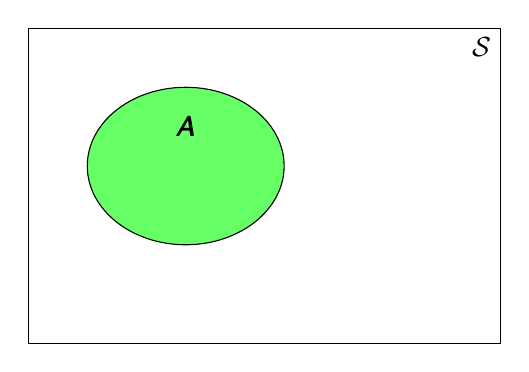
\begin{tikzpicture}
\draw (0,0) rectangle (6,4);
\draw [fill=green!60] (2,2.25) ellipse (1.25cm and 1cm);
\node at (6,4) [below left] {$\mathcal{S}$};
\node at (2,2.75) {$\pmb{A}$};
\end{tikzpicture}
\end{center}

\vfill 

\begin{tcolorbox}[colframe=green!20!black, colback = green!30!white,title=\textbf{Probability}]
\textbf{Probability} is a measure of the likelihood of an event occurring.
\end{tcolorbox}
\vspace{0.25in}

\begin{center}
Probability = $\dfrac{\text{number of ways the event can occur}}{\text{total number of outcomes in sample space}}$
\end{center}

\newpage 


\begin{example}
Determine the probability of each event.
\begin{enumerate}[(a)]
    \item Flipping a coin and landing on heads  \vfill 
    \item Rolling a number less than 3 on a single die \vfill 
    \item Drawing a face card (jack, queen, or king) from a standard deck \vfill 
    \item The number of students in each class at a college is shown in the table below.  
\begin{center}
\begin{tabular}{cccc}
Freshmen	&	Sophomore	&	Junior	&	Senior	\\	\hline
1670		&	2017		&	2975	&	3026	
\end{tabular}
\end{center}
Find the probability that a randomly selected student is a sophomore. \vfill 
    \item The 36 possible sums from rolling 2 dice are shown below.
\begin{center}
\begin{tabular}{c|cccccc}
			&	\textbf{1}	&	\textbf{2}	&	\textbf{3}	&	\textbf{4}	&	\textbf{5}	&	\textbf{6}	\\ \hline
\textbf{1}	&		2		&		3		&		4		&		5		&		6		&		7		\\
\textbf{2}	&		3		&		4		&		5		&		6		&		7		&		8		\\
\textbf{3}	&		4		&		5		&		6		&		7		&		8		&		9		\\
\textbf{4}	&		5		&		6		&		7		&		8		&		9		&		10		\\
\textbf{5}	&		6		&		7		&		8		&		9		&		10		&		11		\\
\textbf{6}	&		7		&		8		&		9		&		10		&		11		&		12
\end{tabular}
\end{center}

What is the probability of rolling a sum of 7?
\end{enumerate}
\end{example}

\vspace{0.5in}
\newpage 

\subsection*{Types of Probability}

\vspace{0.25in}

\begin{itemize}
    \item Classical (a.k.a. \textit{theoretical}) $\longrightarrow$ each outcome has an equal chance of being selected.
    \item Experimental $\longrightarrow$ based on events that have actually occurred.
    \item Subjective $\longrightarrow$ based on opinion
\end{itemize}

\vfill 

\begin{example}
Identify each of the following as experimental probability or subjective probability.
\begin{enumerate}[(a)]
    \item To determine if a coin is fair, it is flipped 100 times and tails occurs 46 times.    \vspace{0.5in}
    \item Your uncle says there is a 95\% chance that Amazon's stock price will go up.
\end{enumerate}
\end{example}

\vfill 

\begin{tcolorbox}[colframe=green!20!black, colback = green!30!white,title=\textbf{Law of Large Numbers}]
As the number of events increases, the experimental probability of an event will approach the classical (theoretical) probability.
\end{tcolorbox}
\vspace{0.25in}

As you flip a fair coin more and more times, $P(\text{tails}) \rightarrow \frac{1}{2}$.

\vfill 

\subsection*{Rules of Probability Club}

\begin{enumerate}
	\item Each probability must be a value between 0 and 1, inclusive.
	\begin{itemize}
		\item A probability of 0 is an \textit{impossible event}.
		\item A probability of 1 is a \textit{certain event}.
	\end{itemize}
	\item The sum of all possible probabilities of a sample space must equal 1.
\end{enumerate}

\end{document}
